\documentclass[]{article}

\usepackage{lipsum}
\usepackage[margin=1in]{geometry}
\usepackage{graphicx} %Allows you to import images
\usepackage{float} %Allows for control of float positions
\begin{document}

\title{Seneka App\\
Universidad de los Andes\\
Airbus Fly Your Ideas}
\author{Garzón Miguel, Gómez Paula, Mendoza Santiago, Villegas Juan}
\maketitle


\Large{
\textbf{1. Summary}\\
}
Seneka is a platform with the ability of integrating the basic technology and engineering concepts in order to provide to the flight passengers the capacity of using their time in a pleasant way along the different airports that might be involved in their path during their business or leisure flights. Moreover, the platform brings support to the airport and airlines to allow them tracking, alerting and making contact with a passenger to notify about changes on their flight itinerary. Seneka also supports the interaction between passenger and the airport, a passenger can get notifications about the commercial offerings and the status of his order. Additionally, the passenger becomes an active member of the security team of the airport by informing to the local authorities about any emergency or misbehaviour from any other person using the app. The application has a sign-in interface for user that subsequently directs it to an airport selection interface where he or she will indicate where they want to be located and find optimal routes for their displacement. Likewise, the app has a search selection interface where the users can find stores, boarding gates and places of interest. Furthermore, an user profile interface can be found where it is possible to identify and modify their personal information and verify their flights.\\
%Seneka app is an App with the ability of integrating the basic technology and engineering concepts in order to provide to the users the capacity of using their time in a pleasant way along the different airports that might be involved in their path during their business or leisure flights. The application has a sign-in interface for user that subsequently directs it to an airport selection interface where he or she will indicate to the application where they want to be located and find optimal routes for their displacement. Likewise, the app has a search selection interface where the users can find stores, boarding gates and places of interest. Furthermore, an user profile interface can be found in the application where it is possible to identify and modify their personal information and verify their flights.

%Seneka app es una plataforma que integra los conceptos básicos de ingeniería y tecnología, para proveer al usuario la capacidad de usar su tiempo de manera placentera en los diferentes aeropuertos que estén involucrados en su recorrido, durante sus vuelos de negocios o diversión. Por otra parte, la plataforma da soporte al aeropuerto y aerolineas permitiendo el seguimiento, alertar y establecer comunicacion con un pasajero para informar acerca de cambios en el intinerario. Seneka también mejora la interaccion entre el pasajero de viaje y los locales comerciales de un aeropuerto, un pasajero puede será notificado acerca de las odertas comerciales y estado de su orden de compra. La aplicación cuenta con una interfaz de inicio de sesión para el usuario que posteriormente lo direcciona a una interfaz de selección de aeropuerto donde este, le indicará a la aplicación cuál es el lugar en el que desea ubicarse y encontrar rutas optimas para su desplazamiento. Así mismo, cuenta con una sección de búsqueda donde puede encontrar tiendas, puertas de embarque y lugares de interés. Conjuntamente, se puede encontrar en la aplicación una interfaz del perfil de usuario en donde este podrá ver, modificar sus datos personales y verificar sus vuelos.
%Seneka app es una aplicación que integra los conceptos básicos de ingeniería y tecnología, para proveer al usuario la capacidad de usar su tiempo de manera placentera en los diferentes aeropuertos que estén involucrados en su recorrido, durante sus vuelos de negocios o diversión. La aplicación cuenta con una interfaz de inicio de sesión para el usuario que posteriormente lo direcciona a una interfaz de selección de aeropuerto donde este, le indicará a la aplicación cuál es el lugar en el que desea ubicarse y encontrar rutas optimas para su desplazamiento. Así mismo, cuenta con una sección de búsqueda donde puede encontrar tiendas, puertas de embarque y lugares de interés. Conjuntamente, se puede encontrar en la aplicación una interfaz del perfil de usuario en donde este podrá ver, modificar sus datos personales y verificar sus vuelos.

\begin{figure}[H]
\centering
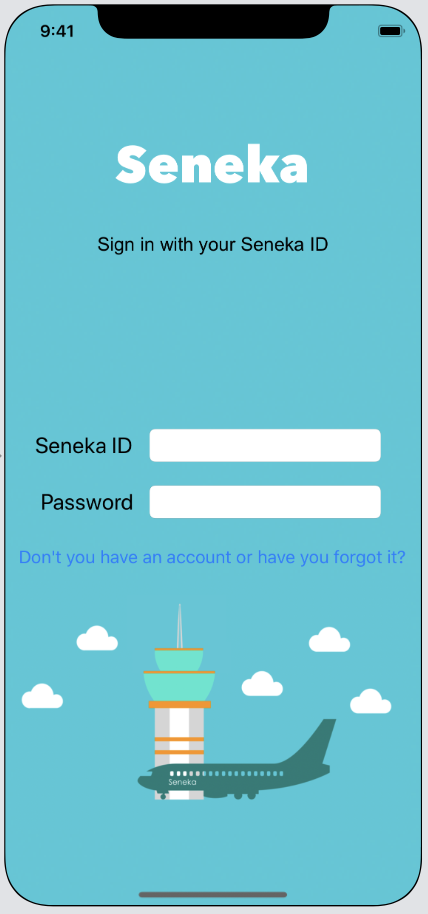
\includegraphics[height=4.0in]{Figura_1.jpg}
\end{figure}

\Large{
\textbf{2. Objetives}\\
}

\Large{
\textbf{2.1 Main Objetive}\\
}\\
[0.1cm]

Design a platform that can provide user support on his/her way through an airport by alerting, giving advice and a guidance through his/her corresponding routes within the airport, while giving secure communication channels between airports, airlines and passengers.\\
%Design an application that can provide to the user a spaces location system and their corresponding routes within the airport.\\

\Large{
\textbf{2.1 Round 2 Specific Objetives}\\
}
\begin{itemize}
	\item Design the business architecture which is consisted of the business canvas and the business ecosystem and the services brochure.
	\item Validate the acceptance of the idea throughout a market analysis based on surveys, existing companies and their success key factors.
	\item Create a sign-in interface based on the results of the design analysis. 
	\item Develop a broaden knowledge of the technical specifications for the mapping and location of the user. 
	
\end{itemize}


\end{document}
